%!TEX root = ../report.tex



%%%%%%%%%%%%%%%%%%%%%%%%%%%%%%%%%%%%%%%%%%%%%%%%%%%%%%%%%%%
\chapter{Delanalyse 1: Intern mobilitet og segmentkriterier\label{kap_delanalyse1_deskriptivt}}
%%%%%%%%%%%%%%%%%%%%%%%%%%%%%%%%%%%%%%%%%%%%%%%%%%%%%%%%%%%

Dette kapitel har tre formål. Det første er at redegøre for dannelsen af de klynger, det danske arbejdsmarked består af, baseret på den jobmobiliteten mellem dem. Det andet er en vurdering kvaliteten af denne klyngedannelse, så mit første undersøgelsesspørgsmål kan besvares: \emph{Er der en opdeling af det danske arbejdsmarkede i delmarkeder, hvor mobilitet indenfor delmarkederne er hyppig, og mellem delmarkederne sjælden?}

Det sidste formål at beskrive hvilke sociale logikker, der kan ses i den struktur, jobmobiliten viser på arbejdsmarkedet. Det leder hen mod delanalyse 2, hvori forskningsspørgsmål 2 søges besvares: Kan det påvises, at der er forskelle i de sociale processer, der foregår i disse delmarkeder? I så er der tale om \emph{segmenter}, og ikke bare delmarkeder, ifølge Bojes segmenteringsteori.  % skal måske ikke stå her

% fra møde med Søren:
% 	Relater til forskningsspm 1, sig hvad du vil gøre (det står sort på hvidt i forskningsspm 1,)
	
% 	skriv hvorfor det giver mening at reducere yderligere, så vi kan gå fra 274 kategorier til 51, uden at tabe intern mob, den er hele tiden sådan at "mobilitet i delmarkeder er hyppig og mellem mindre hyppig", selvom den "går lidt i stå" på de sidste 2 niveauer. Det betyder fremfor at have bygnings-arbejdere har vi en bygge-klynge. Arbejdslogik (slut evt af med det også så du kan lede det frem til delanalyse 2)

	% flere sections/sections så det ikke er så teksttungt i visse afsnit.	

	%  når der tales om et kluster skal der altid et billed med. 


%  delanalyse 2: forskelle i sociale processer: Brug løn, køn, indkomst. Bare start med den, med de lette klynger, fx fra Sørens speciale. 
% 
% 
% Sæt metodeafsnit ind uden tekst, bare "det her er og der er styr på det, du behøver ikke læse det"
% 
% 
% 





% delanalyse 3: Lav forskningsspm 3 om fra: Kan forskelle i de sociale processer vise, at der er tale om segmenter, og ikke blot delmarkeder? Hvordan kommer disse sociale processer til udtryk,  og kan moderne klassebegreber være en måde at forstå delmarkederne på som udtryk for bestemte diffentieringslogikker? Hvad siger disse diffentieringslogikker 

%  se på Goldtorpe, 
%  se på Oesh, 
%  se på Grusky
%  
% 


%%%%%%%%%%%%%%%%%%%%%%%%%%%%%%%%%%%%%%%%%%%%%%
\section{Segmenteringsprocessen \label{delanalyse1_segmenteringsprocessen}}
%%%%%%%%%%%%%%%%%%%%%%%%%%%%%%%%%%%%%%%%%%%%%%

De følgende netværkskort benytter den i kapitel ?? \#todo omtalte metode til at aggregere erhvervskategorier i klynger, baseret på deres mobilitetsmønstre. For at klyngerne kan siges at være egentlige delmarkeder, i Bojes definition, bør der eksistere barrierer for jobmobilitet mellem klyngerne. Vi vil derfor undersøge, om det er tilfældet, og vi starter med en sammenligning af jobmobilitet og antallet af noder i klyngedannelsen. 

Moneca var i stand til at skabe klynger frem til et 5. aggregatniveau. Tabel \ref{tab_delanalyse1_karakteristika}  er et overblik over segmenteringsprocessen, med den gennemsnitlige interne og eksterne mobilitet i klyngerne, for hver segmenteringsniveau.

% 
\begin{table}[H] \centering
\caption{Karakteristika for segmenteringsprocessen}
\label{tab_delanalyse1_karakteristika}
\resizebox{.8\textwidth}{!}{%
\begin{tabular}{@{}l|rrrrr@{}}
Niveau	&	1. niveau	&	2. niveau	&	3. niveau	&	4. niveau	&	5. niveau	\\		\midrule
Antal segmenter	&	273	&	114	&	68	&	53	&	51	\\		
Reduktion i antal segmenter	&	-	&	139\%	&	68\%	&	28\%	&	4\%	\\		\midrule
Intern mobilitet (gns.)	&	68\%	&	75\%	&	77\%	&	78\%	&	79\%	\\		
Ekstern mobilitet (gns.)	&	32\%	&	25\%	&	23\%	&	22\%	&	21\%	\\		\midrule
Mobilitet i alt	&	100\%	&	100\%	&	100\%	&	100\%	&	100\%	\\		
Forøgelse i intern mobilitet	&	-	&	10\%	&	3\%	&	2\%	&	1\%	\\		\midrule
\end{tabular} }
\end{table}
%

Det første iøjnefaldende er at den interne mobilitet på det (uaggregerede) niveau 1 er højt i sig selv: 68 \%. Det indikerer at en væsentlig mængde skift foregår på et meget lavt \texttt{DISCO}-niveau. Langt de fleste bliver indenfor deres eget job. Eller ihvertfald et job, der ligger så tæt på, at man selv på mit usædvanligt lave \texttt{ISCO}-niveau ikke kan skelne dem fra hinanden.

Den mest markante aggregering i klynger og stigning i intern jobmobilitet finder sted i skiftet fra 1. niveau til 2. niveau, og herefter falder effekten af klyngedannelsen på den interne jobmobilitet støt. Sideløbende med gennemgangen tabel \ref{tab_delanalyse1_karakteristika} fra niveau til niveau, optræder en visuel repræsentation af samme. Forskellen på hvide og sorte noder i figurerne på side \pageref{fig_delanalyse1_kort_seg_proces2} til side \pageref{fig_delanalyse1_kort_seg_proces5} er simpel. Sorte node indikerer at denne node er blevet inkluderet i en ny klynge siden det foregående niveau. Hvid node indikerer at den \emph{ikke} er blevet inkluderet i en ny klynge siden niveauet før. 
Jeg har ikke afbilledet niveau 1, da der ikke findes et foregående niveau at vise et skift \emph{fra}. 

\begin{wrapfigure}{r}{8cm}
  \vspace{-20pt}
  \begin{center}
   \caption{}
   \label{fig_delanalyse1_kort_seg_proces2}
    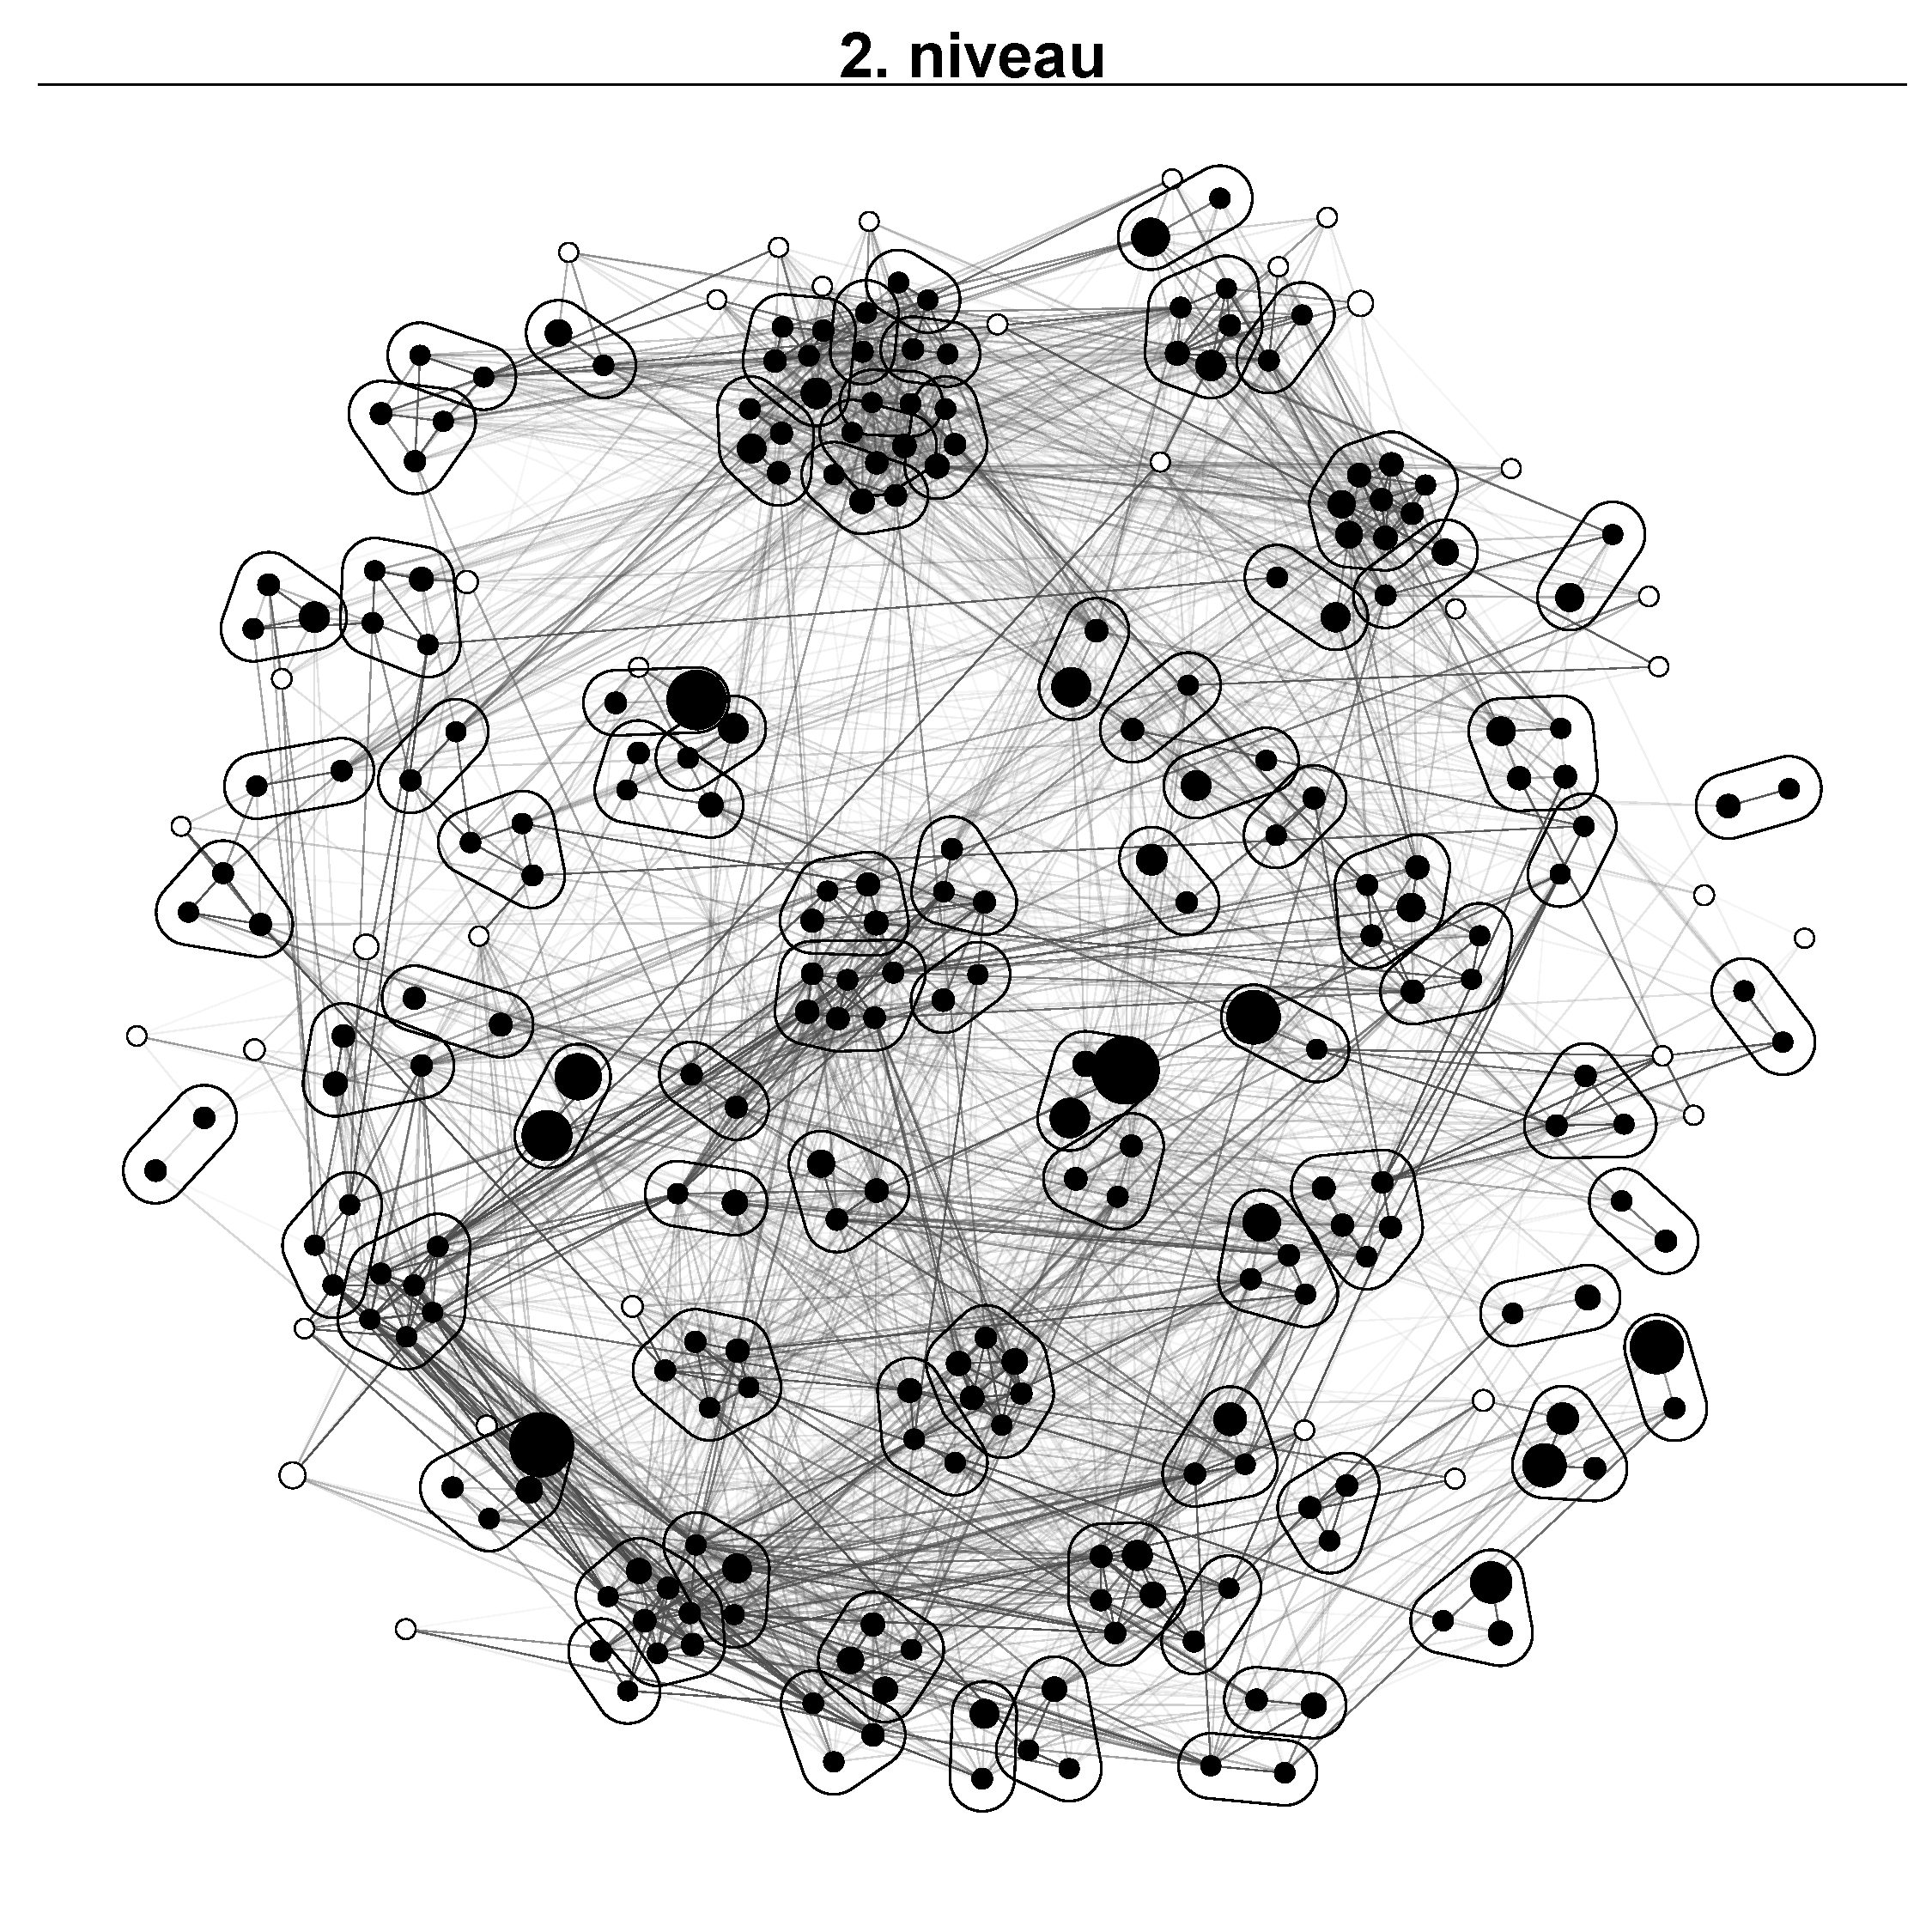
\includegraphics[width=8cm]{fig/netvaerkskort/kort_seg_proces2.pdf}
  \end{center}
  \vspace{-20pt}
\end{wrapfigure}
%

\underline{På 2. niveau} går vi fra de oprindelige 273 fritstående noder til 81 klynger, samt 33 endnu fritstående noder. Det vil sige 114 grupper i alt. Der skelnes i ovenstående tabel ikke mellem enkelte noder og klynger, da klyngernes interne mobilitet jo netop skal erstatte nodernes, og en direkte sammenligning derfor er ønskelig.
Vi ser ud fra tabel \ref{tab_delanalyse1_karakteristika} at på 2. niveau er antallet af noder reduceret med 139 \%, og den gennemsnitlige interne mobilitet i segmenterne er steget med 7 procentpoint, svarende til en forøgelse på 10 \%. 

\begin{wrapfigure}{l}{8cm}
  \vspace{-20pt}
  \begin{center}
   \caption{}
   \label{fig_delanalyse1_kort_seg_proces3}
    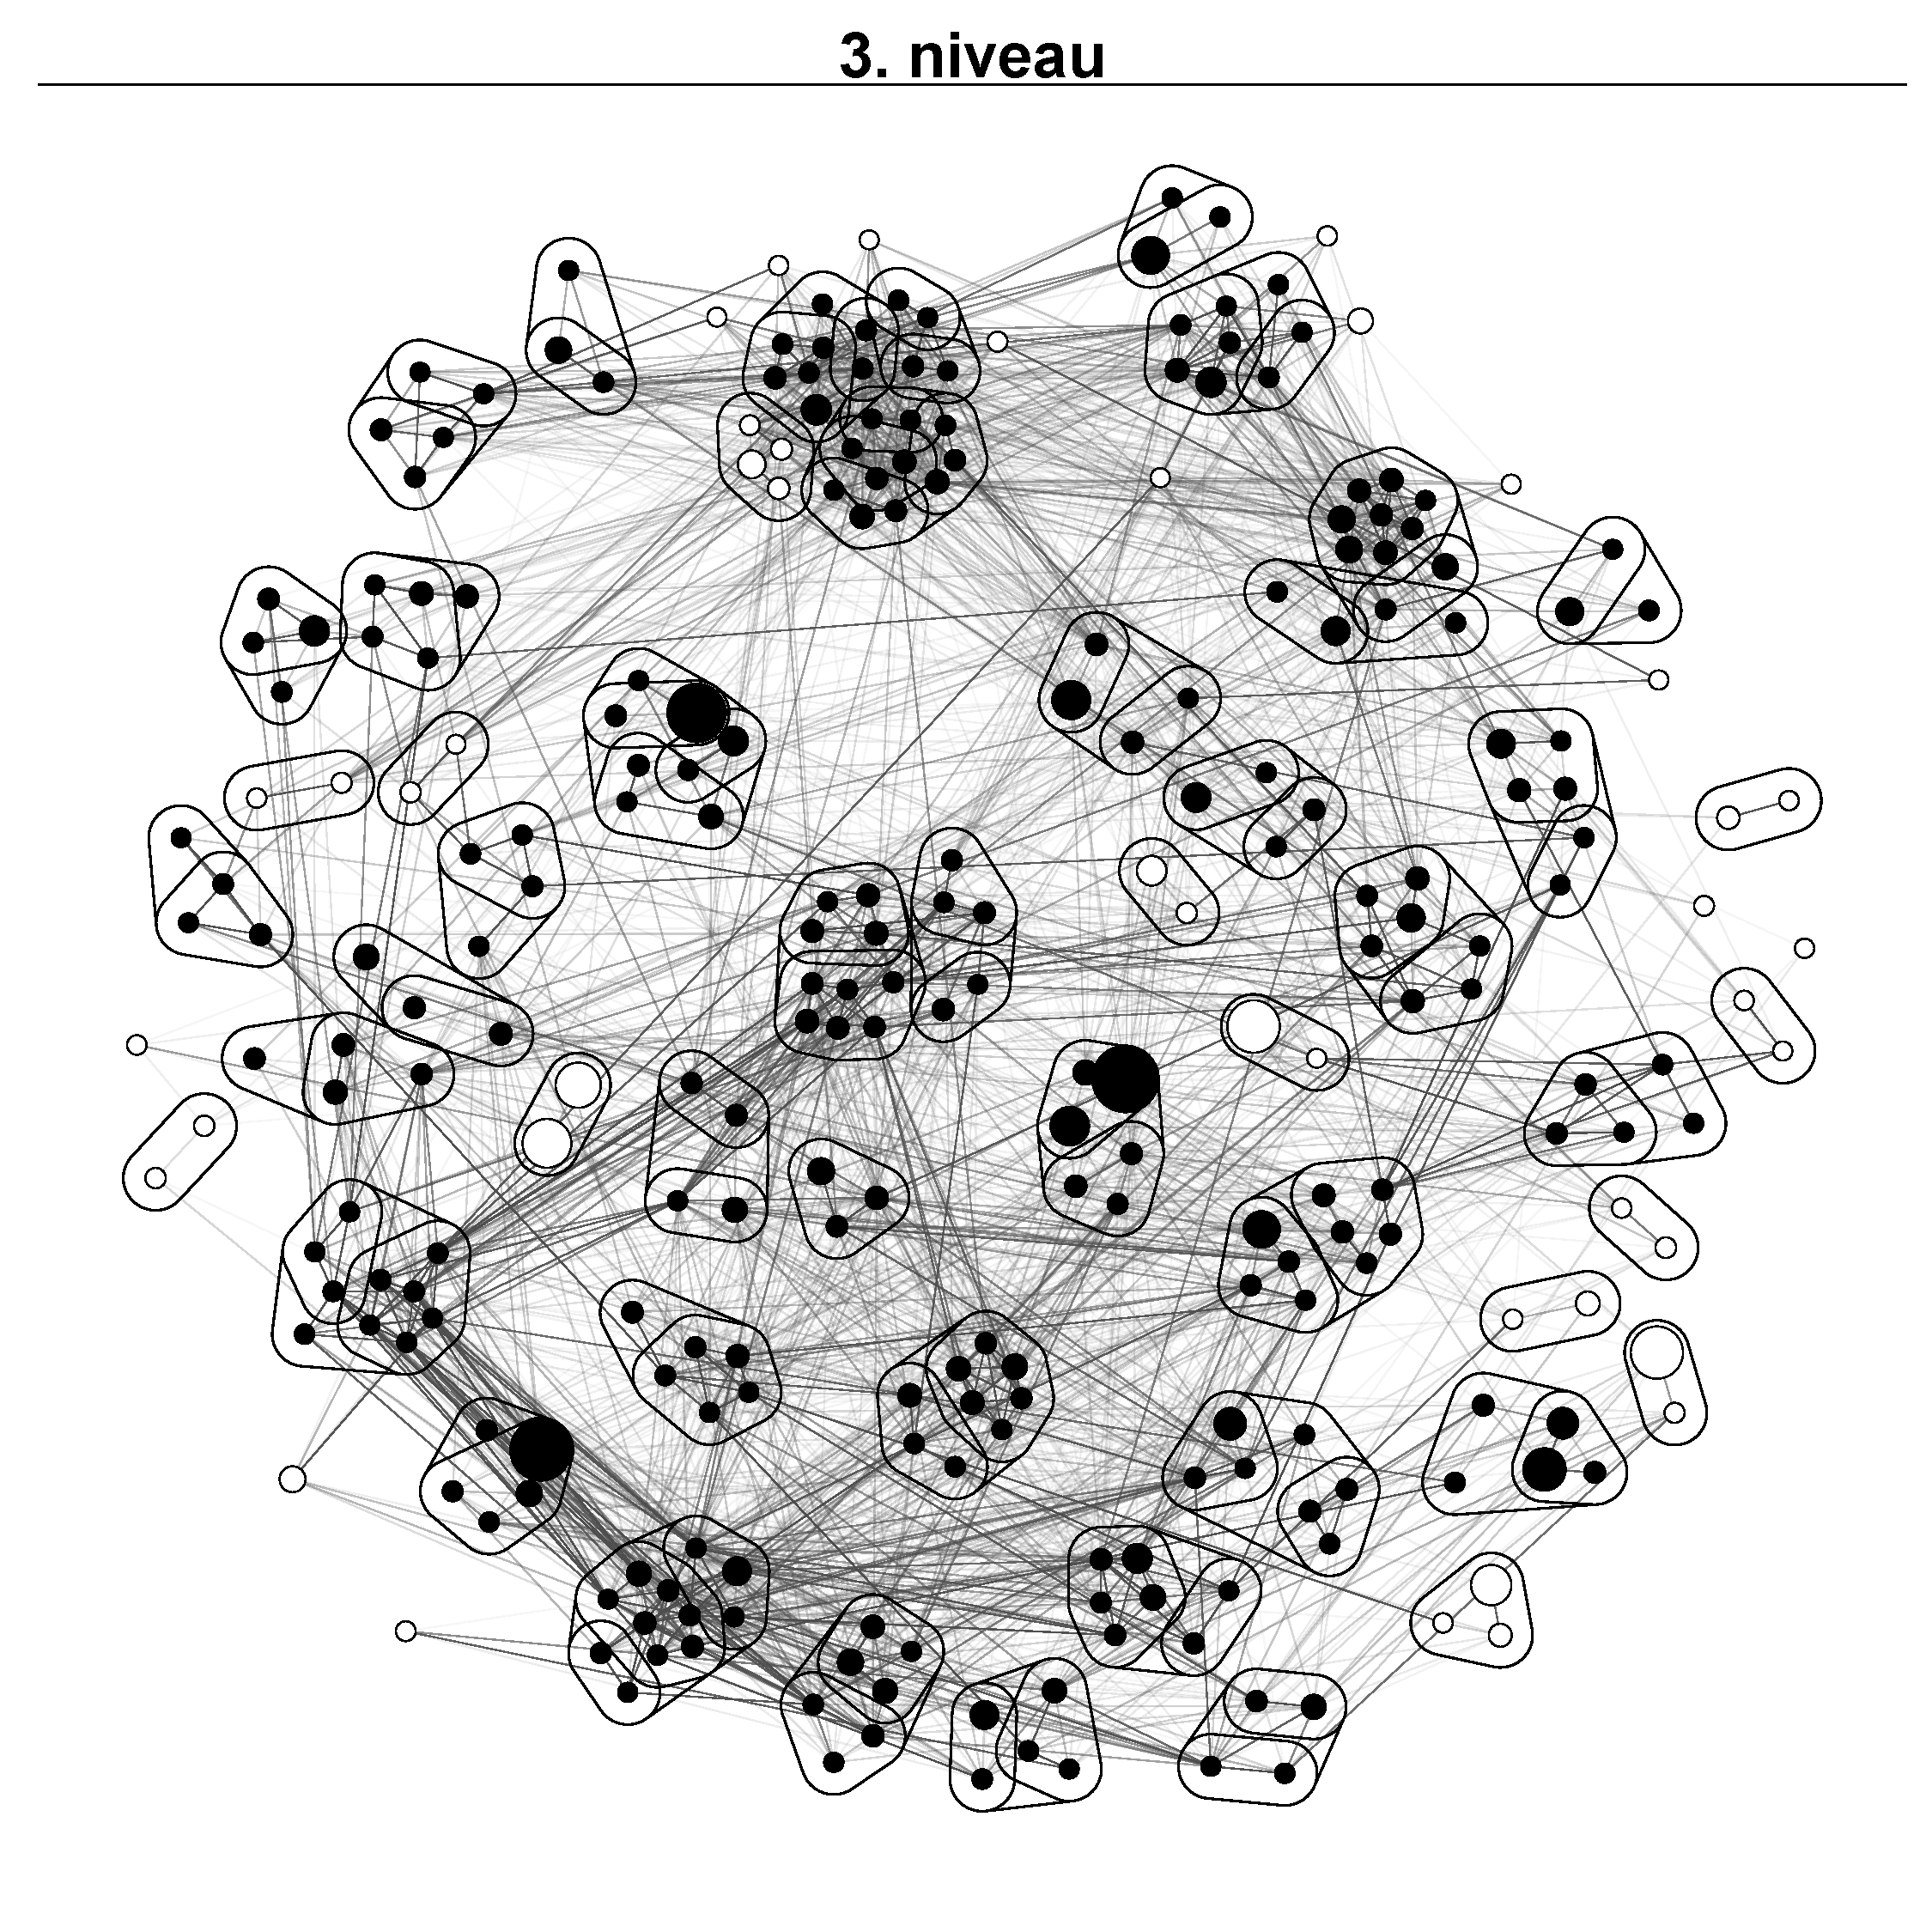
\includegraphics[width=8cm]{fig/netvaerkskort/kort_seg_proces3.pdf}
  \end{center}
  \vspace{-20pt}
\end{wrapfigure}

\underline{På 3. niveau}, afbilledet i figur \ref{fig_delanalyse1_kort_seg_proces3}, inkluderes 21 enkeltstående noder i klynger, samt en række niveau 2 klynger aggrereres yderligere. Det reducerer antallet af grupper til 68. Det ses ud fra tabellen at stigningen i den gennemsnitlige interne mobilitet kun er på 2 procentpoint, svarende til 2,5 \%. Tilgengæld er reduktionen i antallet af grupper på 68 \%. Det vil sige at kompleksiteten i netværket reduceres, uden at det går udover den interne mobilitet, der er stigende, omend svagt. Det er tendensen fra niveau 3 og frem: Der foretages stadig væsentlige sammenlægninger af klynger og noder til større klynger, men betydning af sammenlægningen på den interne mobilitet er markant faldende. Det ser jeg som udtryk for, at jo længere væk fra den sociale kontekst af det oprindelige job, vi kommer, desto mindre systematik er der i jobskiftet.

\begin{wrapfigure}{l}{8cm}
  \vspace{-20pt}
  \begin{center}
    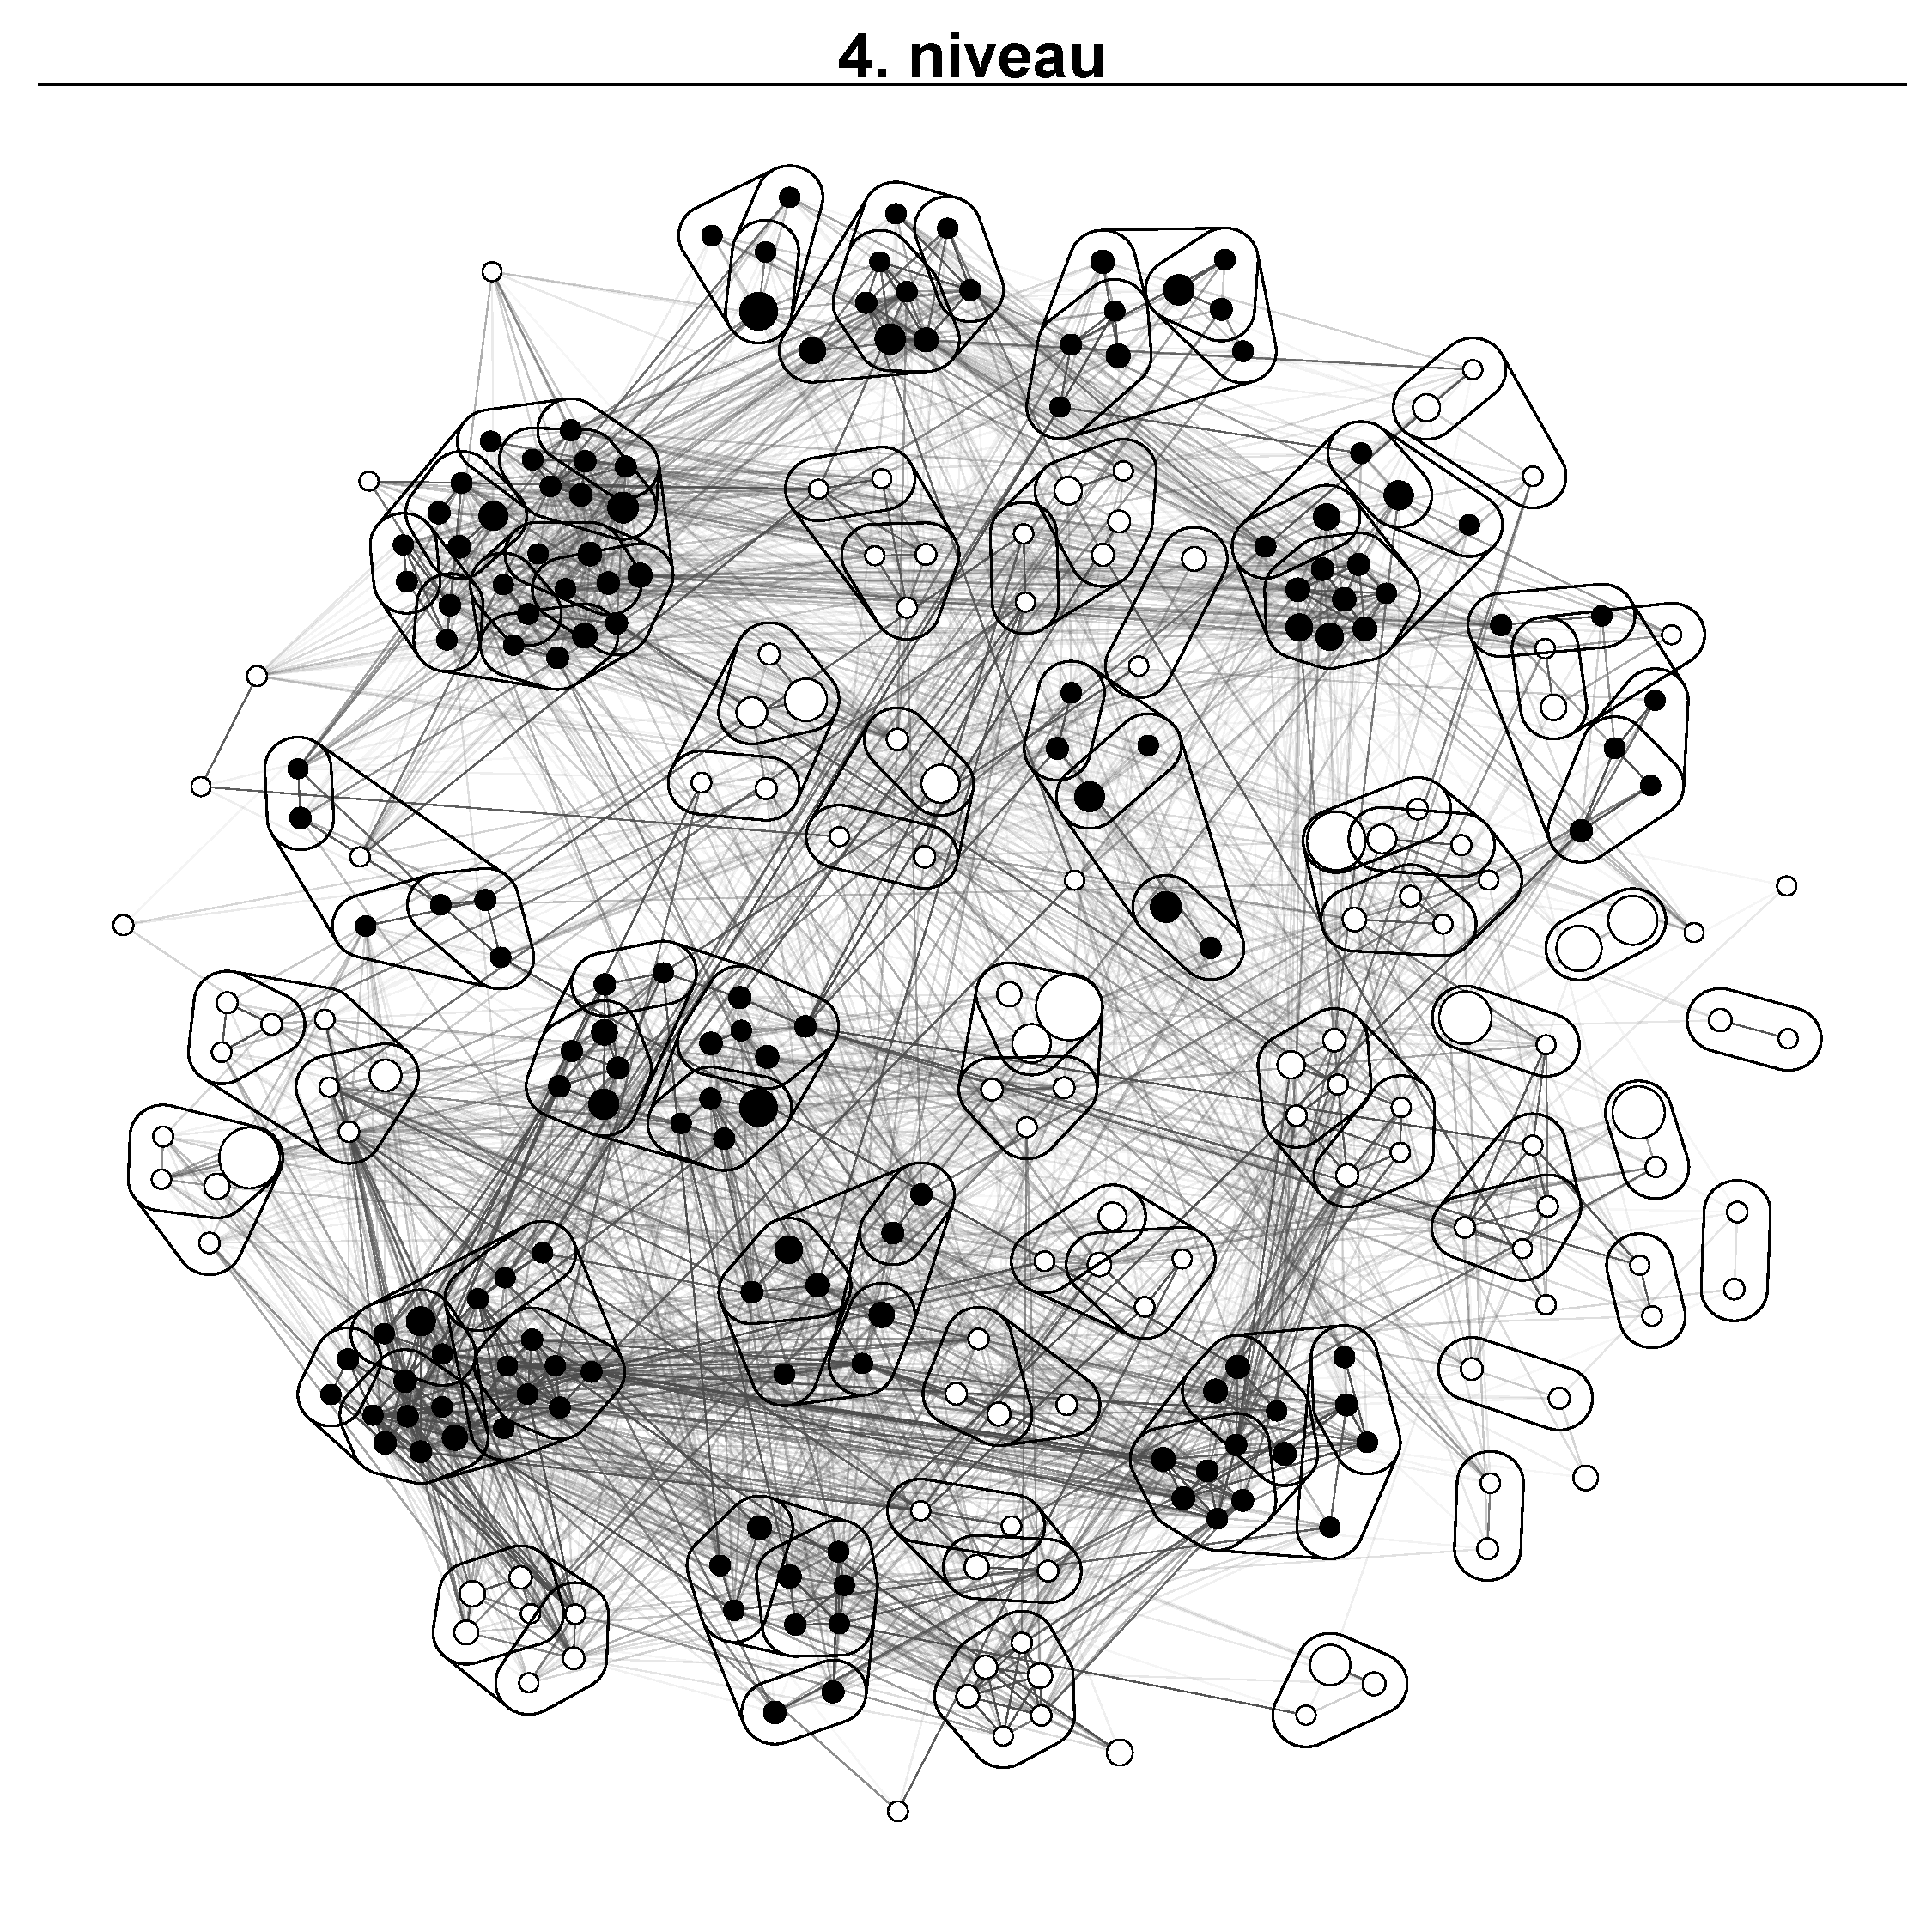
\includegraphics[width=8cm]{fig/netvaerkskort/kort_seg_proces4.pdf}
   \caption{}
   \label{fig_delanalyse1_kort_seg_proces4}
  \end{center}
  \vspace{-20pt}
\end{wrapfigure}

\underline{På 4. niveau} skabes 13 nye klynger. Kun en enkelt af disse sker i en sammenlægning med en enkeltstående node. Resten er tidligere segmentdannelser. Det er på dette niveau, at sammenlægningerne binder allerede store klynger sammen, og vi får udvidede klynger med en betragtelig mængde forskellige arbejdsfunktioner samlet under ét. Disse klynger af arbejdsfunktioner er ikke baseret på en \emph{technicist vision}, som Grusky den advarer imod, og heller ikke en a priori teoretisk opdeling. Men er istedet baseret på den sociale nærhed, der må findes i jobtyper, hvor der foregår “let og typisk” mobilitet mellem dem, som Weber skriver. %kalder det, sin beskrivelse af (et af) de definerende træk ved social klasse: Individuel mobilitet% Det her skal nok stå i teori-afsnittet, og så henvises til her i stedet. \#todo
%
%\footnote{Der er naturligvis flere elementer end individuel jobmobilitet på spil. Det fulde citat lyder: “\textit{A »social class« makes up the totality of those class situations within which individual and generational mobility is easy and typical.}” \parencite[302]{Weber1978}. }%
%
 

De er derimod baseret på reel jobmobilitet m

Hvad jeg argumentere for er social, hverdagsbaseret kontakt, som efterlyst af af Grusky i hans kulturalistiske klassesyn.  Der er nu 53 grupper hvoraf 13 er noder. Den interne mobilitet er steget med et enkelt beskedent procentpoint. Antallet af gruper er tilgengæld reduceret med 28 \%, lidt over $\nicefrac{1}{4}$.

% kunne evt argumentere for hvorfor en 1 procent stigning er ret meget værd: I diverse effektforskninger, fx Stefans, er bare den 1 1/2 procent han kan finde i indkomstforskelle meget. De forklarer ofte kun 5-10 procent af den totale variation. kan ikke overføres direkte, men bare for at sige: 1 procent er ikke nødvendigvis "lidt".

%%%%%%%%%%%%%%%%%%%%%%%%%%%%%%%%%%%%%%%%%%%%%%
\section{Det endelige mobilitetskort \label{delanalyse1_endelige mobilitetskort}}
%%%%%%%%%%%%%%%%%%%%%%%%%%%%%%%%%%%%%%%%%%%%%%

Det endelige kort findes på niveau 5, da Moneca ikke kan aggregere klynger på et højere niveau end det. Vi mindes fra gennemgangen af Moneca-proceduren på side  \pageref{metode_monecastepbystep}, at det betyder, at Moneca ikke kan finde nogle noder eller tidligere klynger, hvor der er intern mobilitet mellem  \emph{alle} klynger fra niveauet tidligere. %check lige op på det med Anton \#todo 
På dette endelige aggregeringsniveau er der en beskeden inklusion af en enkelt node i en niveau 4- klynge, samt en større sammenlægning af en niveau 4- og en niveau 3-klynge. Det bringer os ned på 12 enkeltstående noder, samt 39 klynger. 

\begin{figure}[H]
\begin{centering}
  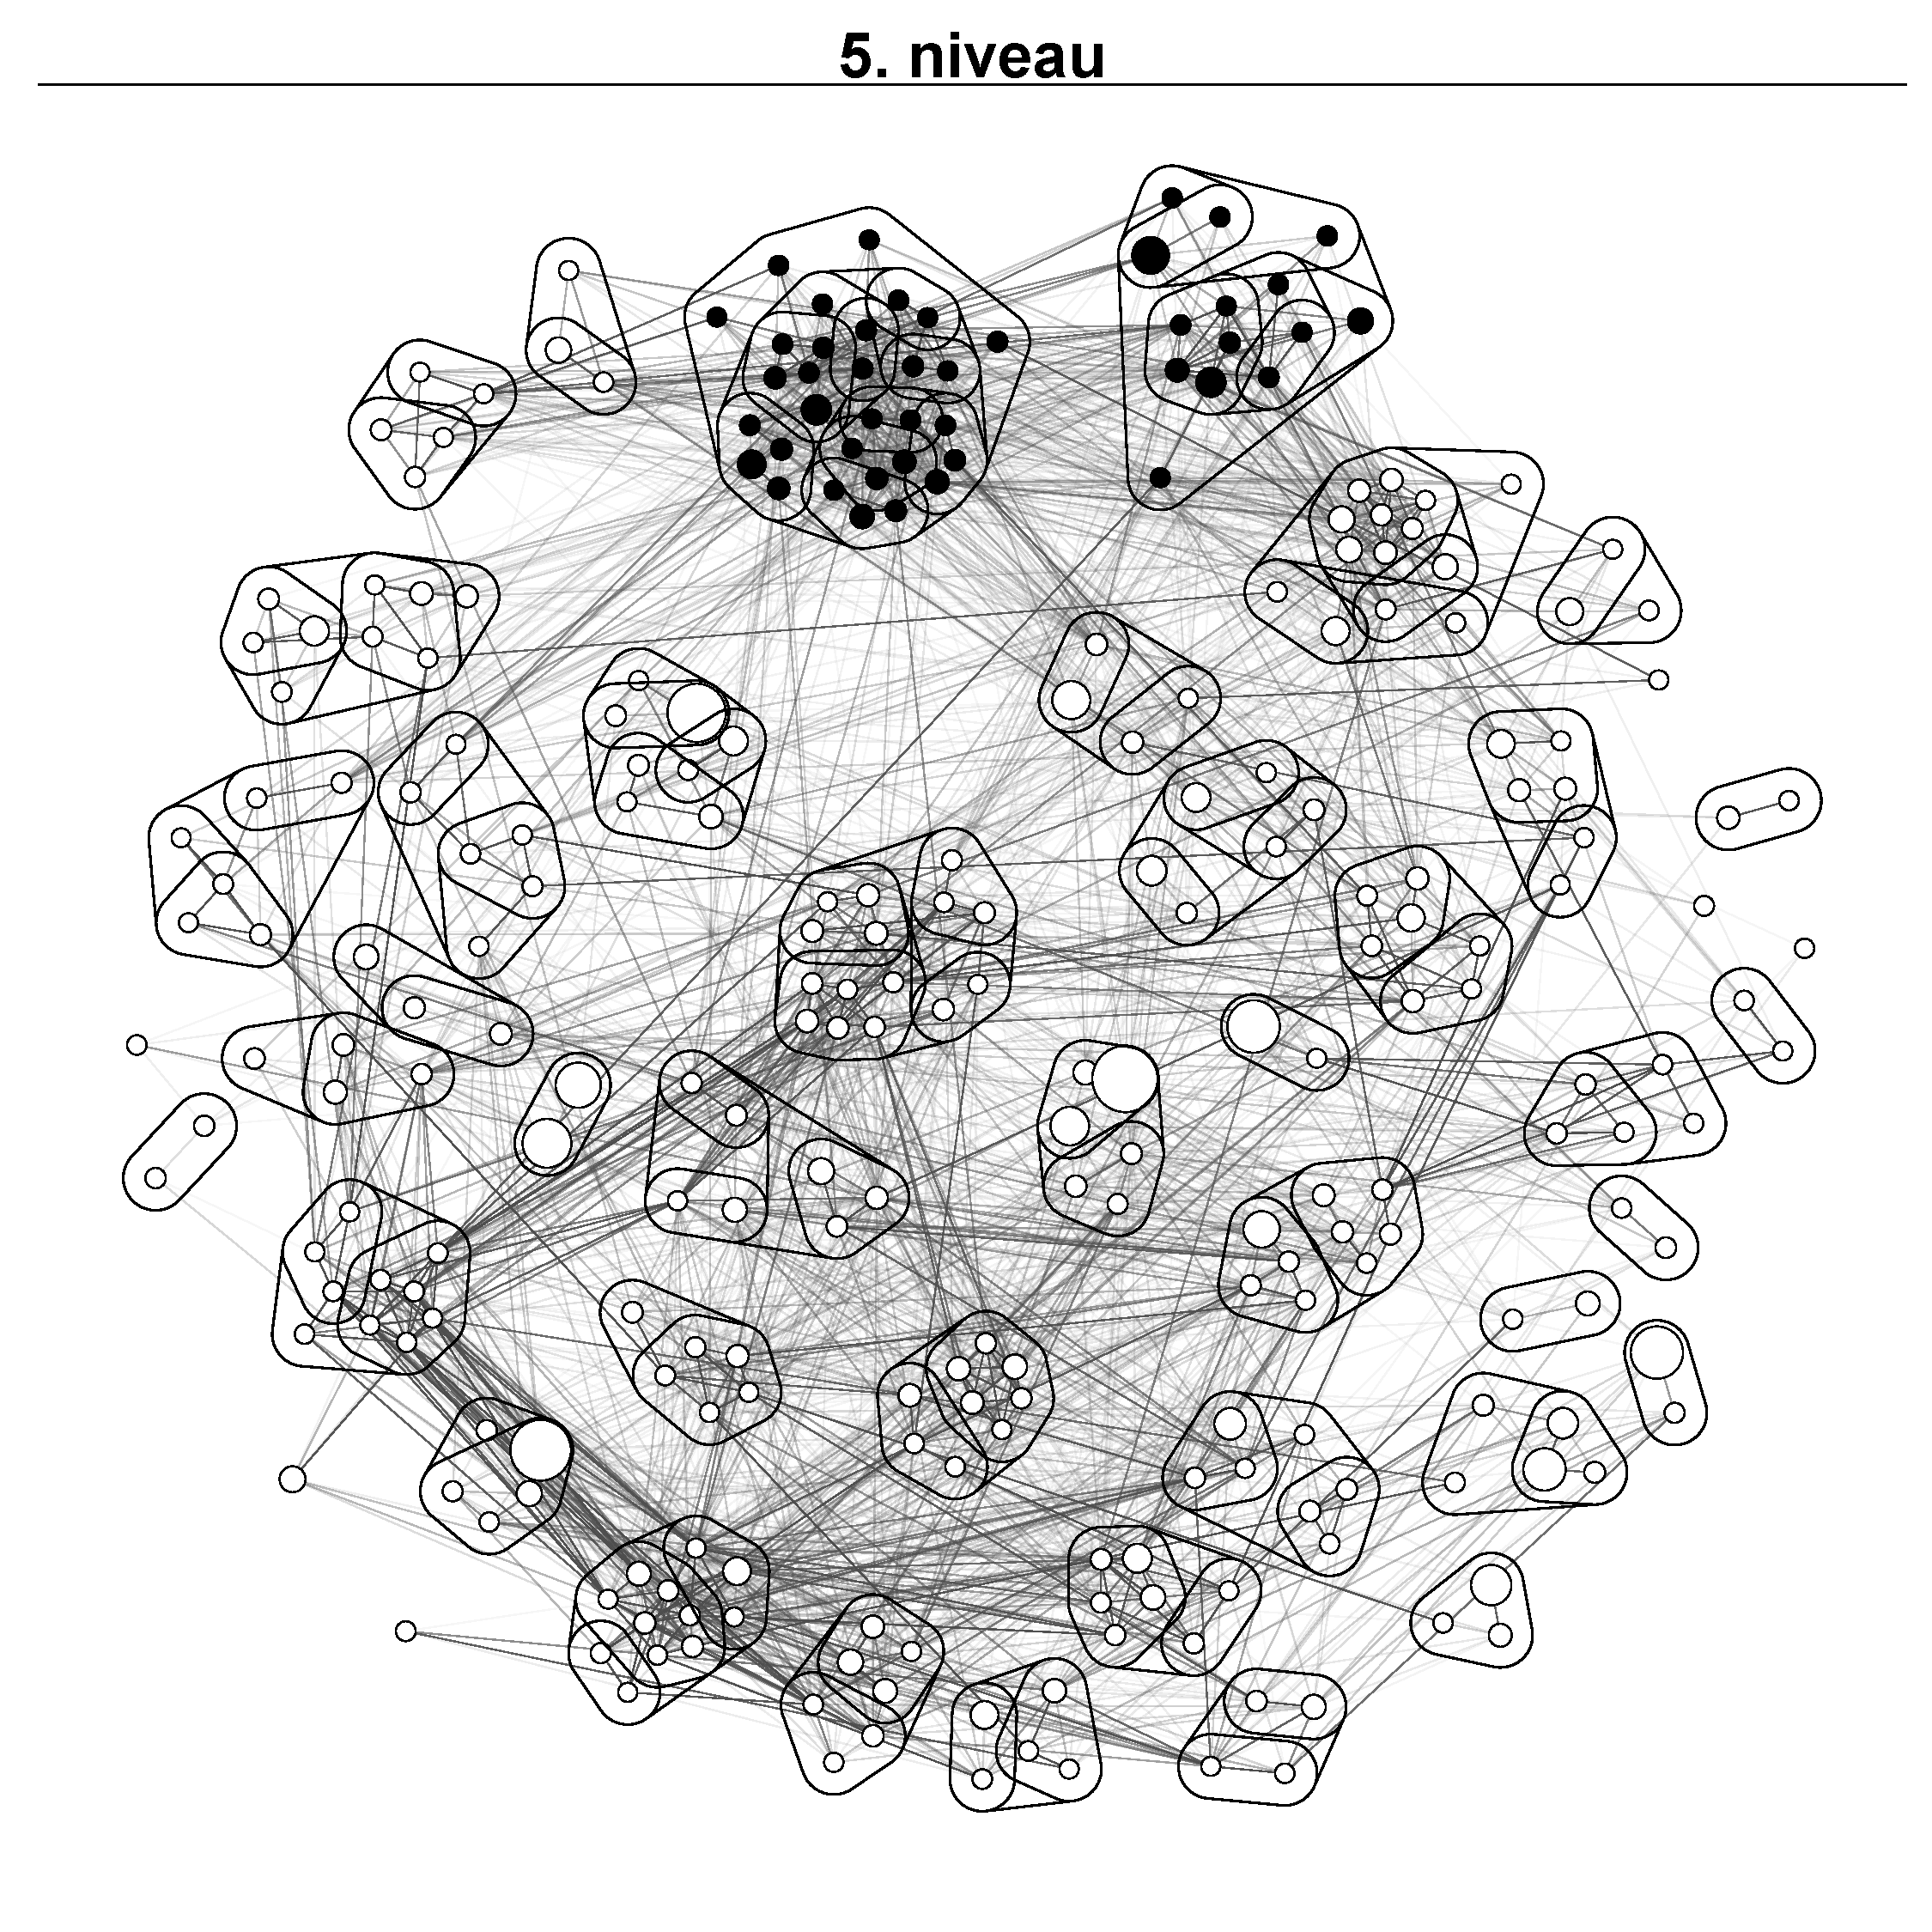
\includegraphics[width=10 cm]{fig/netvaerkskort/kort_seg_proces5.pdf}
  \label{fig_delanalyse1_kort_seg_proces5}
  \caption{}
\end{centering}
\end{figure}

Her er forbedringen i den interne mobilitet endnu en gang på et enkelt procentpoint.  En gennemsnitlig intern mobilitet tæt på 80 \% er hvad det er hvad det er muligt at komme frem til. Dette forekommer rimeligt og acceptabelt, og en stigning på 11 procentpoint i den interne mobilitet fra niveau 1 til niveau 5 vurderer jeg som ganske tilfredsstillende, når det endelige resultat forklarer omtrent $\nicefrac{4}{5}$ af mobiliteten.

Den oprindelige 273 x 273 mobilitetstabel nu er reduceret til en mere overkommelig 51 x 51 mobilitetstabel. Ud af disse 51 kategorier er 12 enkelstående noter, der ikke er sammenlagt med andre noter, mens 39 er klynger. Tabel \ref{tab_delanalyse1_noegletalniveau1og5} viser yderligere centrale mål. Disse viser tydeligt at aggregeringen har skabt færre kategorier med højere intern mobilitet.

%!TEX encoding = UTF-8 Unicode
%!TEX root = ../report.tex
% Table generated by Excel2LaTeX from sheet 'delanalyse1_noegletalniveau1og5'
\begin{table}[htbp]
  \centering
  \caption[Nøgletal for første og sidste niveau i klyngedannelsen]{Nøgletal for (det uaggregerede) niveau 1 og (det endelige) niveau 5}
  \resizebox{.8\textwidth}{!}{%
    \begin{tabular}{lcccccc}
          &       & gns. intern & sd afvigelse  &       &       &  \\
    Niveau & grupper &  mobilitet & 
\emph{\tiny{(i procentpoint)}} & median & min   & max \\
    \midrule
    1. niveau & 273   & 68\%  & 12    & 68\%  & 43\%  & 97\% \\
    5. niveau & 47    & 81\%  & 10    & 80\%  & 54\%  & 96\% \\
    \bottomrule
    \end{tabular}}%
  \label{tab_delanalyse1_noegletalniveau1og5}%
\end{table}%


Medianen på det 1. niveau er på 79 \%, mens det på 5. niveau er steget til 80 \%. Standardafvigelsen for den interne mobilitet på det 1. niveau er på 12 \%, mens den på det 5. niveau er på 10 \%. At standardafvigelsen er faldet og medianen er steget, er vigtigt, fordi det fortæller os at gennemsnittet ikke er trukket op via enkelte klynger.  Det er en generel forbedring af mobilitetsstrukturen. Det ses også ud fra minimumværdierne. Hvor de laveste værdier tidligere lå på lidt over 40 \%, ligger de nu på lidt over 50 \%. På de 3 centrale mål for kontinuerte variable (Find henvisning Malchow-Muller \#todo) er der sket en forbedring. 5. niveau forklarer \emph{mere} mobilitet, og kategoriernes interne mobilitet svinger \emph{mindre} om gennemsnitsmobiliteten end i kategorierne på 1. niveau. Det er meget tilfredsstillende, da det indikerer at et højere aggregeringsniveau ud fra Monecas beslutningsprocedure forklarer \emph{hvor} mobiliteten løber hen, når den bevæger sig udenfor de oprindelige kategorier. 
% Det er jo sådan set også det, den er designet til, kunne man indvende. Men det tilfredsstillende her er at helt op til \emph{det 5. aggregreringsniveau} er der stadig en bedre forklaringskraft end på de tidligere niveauer. Man kunne forestille sig at for mange kompromisser med sammenlægninger - genkald argumentet fra side ??(det om at der lægger noder sammen der rent faktisk ikke hænger sammen \#todo) ville fungere kontraproduktivt over et vist niveau, men det er altså ikke tilfældet. % ved ikke helt om det her argument egentligt holder -vil en større sammenlægning ikke bare automatisk give bedre forklaring? Nej! for hvis en node nu har meget mere udveksling med en node udenfor det, den er lagt sammen med, så ville det jo godt kunne trække ned. Men det sker ikke her, altså er det en god sammenlægning. Tror jeg. 

Fra 3. niveau og frem er klyngedannelsens primære funktion at danne større segmenter, det vil sige reducere kompleksiteten i jobstrukturen. Husk på at det ikke kun betyder at antallet af kategorier falder. Visse kategorier indeholer langt flere beskæftigede end andre, og kan derfor anses som mere væsentlige sammenlægninger. Vi får dermed nogle klynger, der antalsmæssigt beskæftiger store dele af den danske befolkning. Dette vil jeg mene er et andet vigtigt parameter i klyngedannelsen. Det vil ikke blive gennemgået nøje her, og vil istedet blive præsenteret i Delanalyse 2 på side \pageref{kap_delanalyse2_socialeprocesser}.


%%%%%%%%%%%%%%%%%%%%%%%%%%%%%%%%%%%%%%%%%%%%%%
\section{Den interne mobilitet i segmenterne \label{analyse_deskriptivt_within_mob_seg}}
%%%%%%%%%%%%%%%%%%%%%%%%%%%%%%%%%%%%%%%%%%%%%%


Det første netværkskort, jeg vil præsentere, er kortet der viser den interne mobilitet for hvert segment,  i figur \ref{fig_analyse_deskriptivt_kort_intern_mob_seg}, \pref{fig_analyse_deskriptivt_kort_intern_mob_seg}). % Den interne og eksterne mobilitet er drøftet teoretisk i afsnit ?? og den metodiske implementering er drøftet i afsnit ?? \#todo.
Da dette er det første kort, vil jeg først præsentere en vejledning i at læse de informationer, kortet indeholder. 

Noget man måske ligger mærke til ved første øjekast, er forbindelsernes farve og størrelsen af noderne. De vil blive gennemgået her.

\underline{Forbindelsens farve} er udtryk for styrken af forbindelsen. Som beskrevet i afsnit \ref{metode_relativrisiko}, er forbindelsernes styrke målt ved den relative risiko. Et forholdsmål, der udtrykker mobiliteten fra en kategori til en anden, givet den relative størrelse af antallet af beskæftigede i kategorien. Det er styrken af denne relative risiko (RR), der afgør farven på forbindelserne, der kan antage tre nuancer: Helt lysegrå angiver en RR på 3%
%
\footnote{Husk på fortolkningen af relativ risiko:  det vil sige, at der er ved en lysegrå forbindelse er 3 gange så stor sandsynlighed for mobilitet fra den forladte beskæftigelse til den nye beskæftigelse, i forhold til hvis der var tale om et helt frit arbejdsmarked.}%
%
. Helt orange angiver en RR på 15. Helt mørkerød angiver en RR på 30 \emph{ eller derover}. I bestemmelsen af klyngerne, er alle forbindelser med en RR på over 1 medtaget som en forbindelse. På det visuelle kort er den informationsmængde upraktisk. Det bliver umuligt at aflæse den underliggende systematik i hvilke forbindelser, der værd at lægge mærke til. Enkelte forbindelser har RR-værdier på flere tusinde, men de fleste langt lavere: Medianen er på 2,1. En relativ risiko på 3 svarer cirka til den 65. percentil, og 15 er cirka den 90 percentil. 30 svarer til cirka den 92,5'te percentil, og er ikke valgt ud fra denne, men bestemt ud fra det punkt, hvor der sker en eksponentiel stigning i styrken af forbindelser. Derfor skal den rene orange farve tolkes ikke \emph{som} 30, men som voldsomt stærk forbindelse fra én jobtype til en anden. 

\underline{Størrelsen på en node} repræsenterer ganske simpelt hvor mange personer, der i gennemsnit er i beskæftiget indenfor jobkategorien i årrækken 1996-2009%
%
\footnote{Når jeg fra nu af taler om hvor mange der er beskæftigede, er det underforstået at der er tale om det gennemsnitlige antal \emph{indenfor årrækken 1996-2009}, med mindre det eksplicit fremhæves at der er tale om noget andet.}%
%
. Ligesom med forbindelsernes styrke, er der ikke tale om et korrekt repræsenteret størrelsesforhold mellem de forskellige jobkategorier. Den største kategori, \texttt{5220: Ekspedient-, kasse- og demonstrationsarbejde} indeholder 114.869 personer i gennemsnit, svarende til 4,9 \% af det totale antal beskæftigede. Mens den mindste, \texttt{7346: Serigrafisk arbejde} indeholder 504 personer, svarende til 0,02 \% af det totalen. Det er for komplekst til visuel afkodning i et allerede informationstungt netværkskort, da de mindste noder ville blive meget små og de store noder meget store. Derfor har jeg valgt et størrelsesforhold mellem noderne, der ikke er 1:1 med deres reelle forskelle i størrelse, og som alligevel giver en fornuftig fornemmelse for disse størrelsesforhold.  

Man skal dermed se både farve af forbindelserne og nodernes størrelse som en grov målestok af den variabel, den repræsenterer. Med vægten lagt på nem visuel afkodning, fremfor korrekt gengivelse af datakompleksisteten.

Til sidst skal læseren mindes om, at der er tale om et retningsbestemt netværk, hvor pilene på kortet angiver retningen af mobiliteten mellem noderne. 

Det var de generelle retningslinjer for kortene. Dette gælder alle de præsenterede kort. Næste side indeholder(vær sikker på det gør det \#todo) det første kort, farvelagt efter den interne mobilitet på segmentniveau.


\newgeometry{left=-0.01cm,bottom=0.1cm}
\begin{figure}[H]
\begin{center}
	\caption{Intern mobilitet for segmenterne.}
	\label{fig_analyse_deskriptivt_kort_intern_mob_seg}
	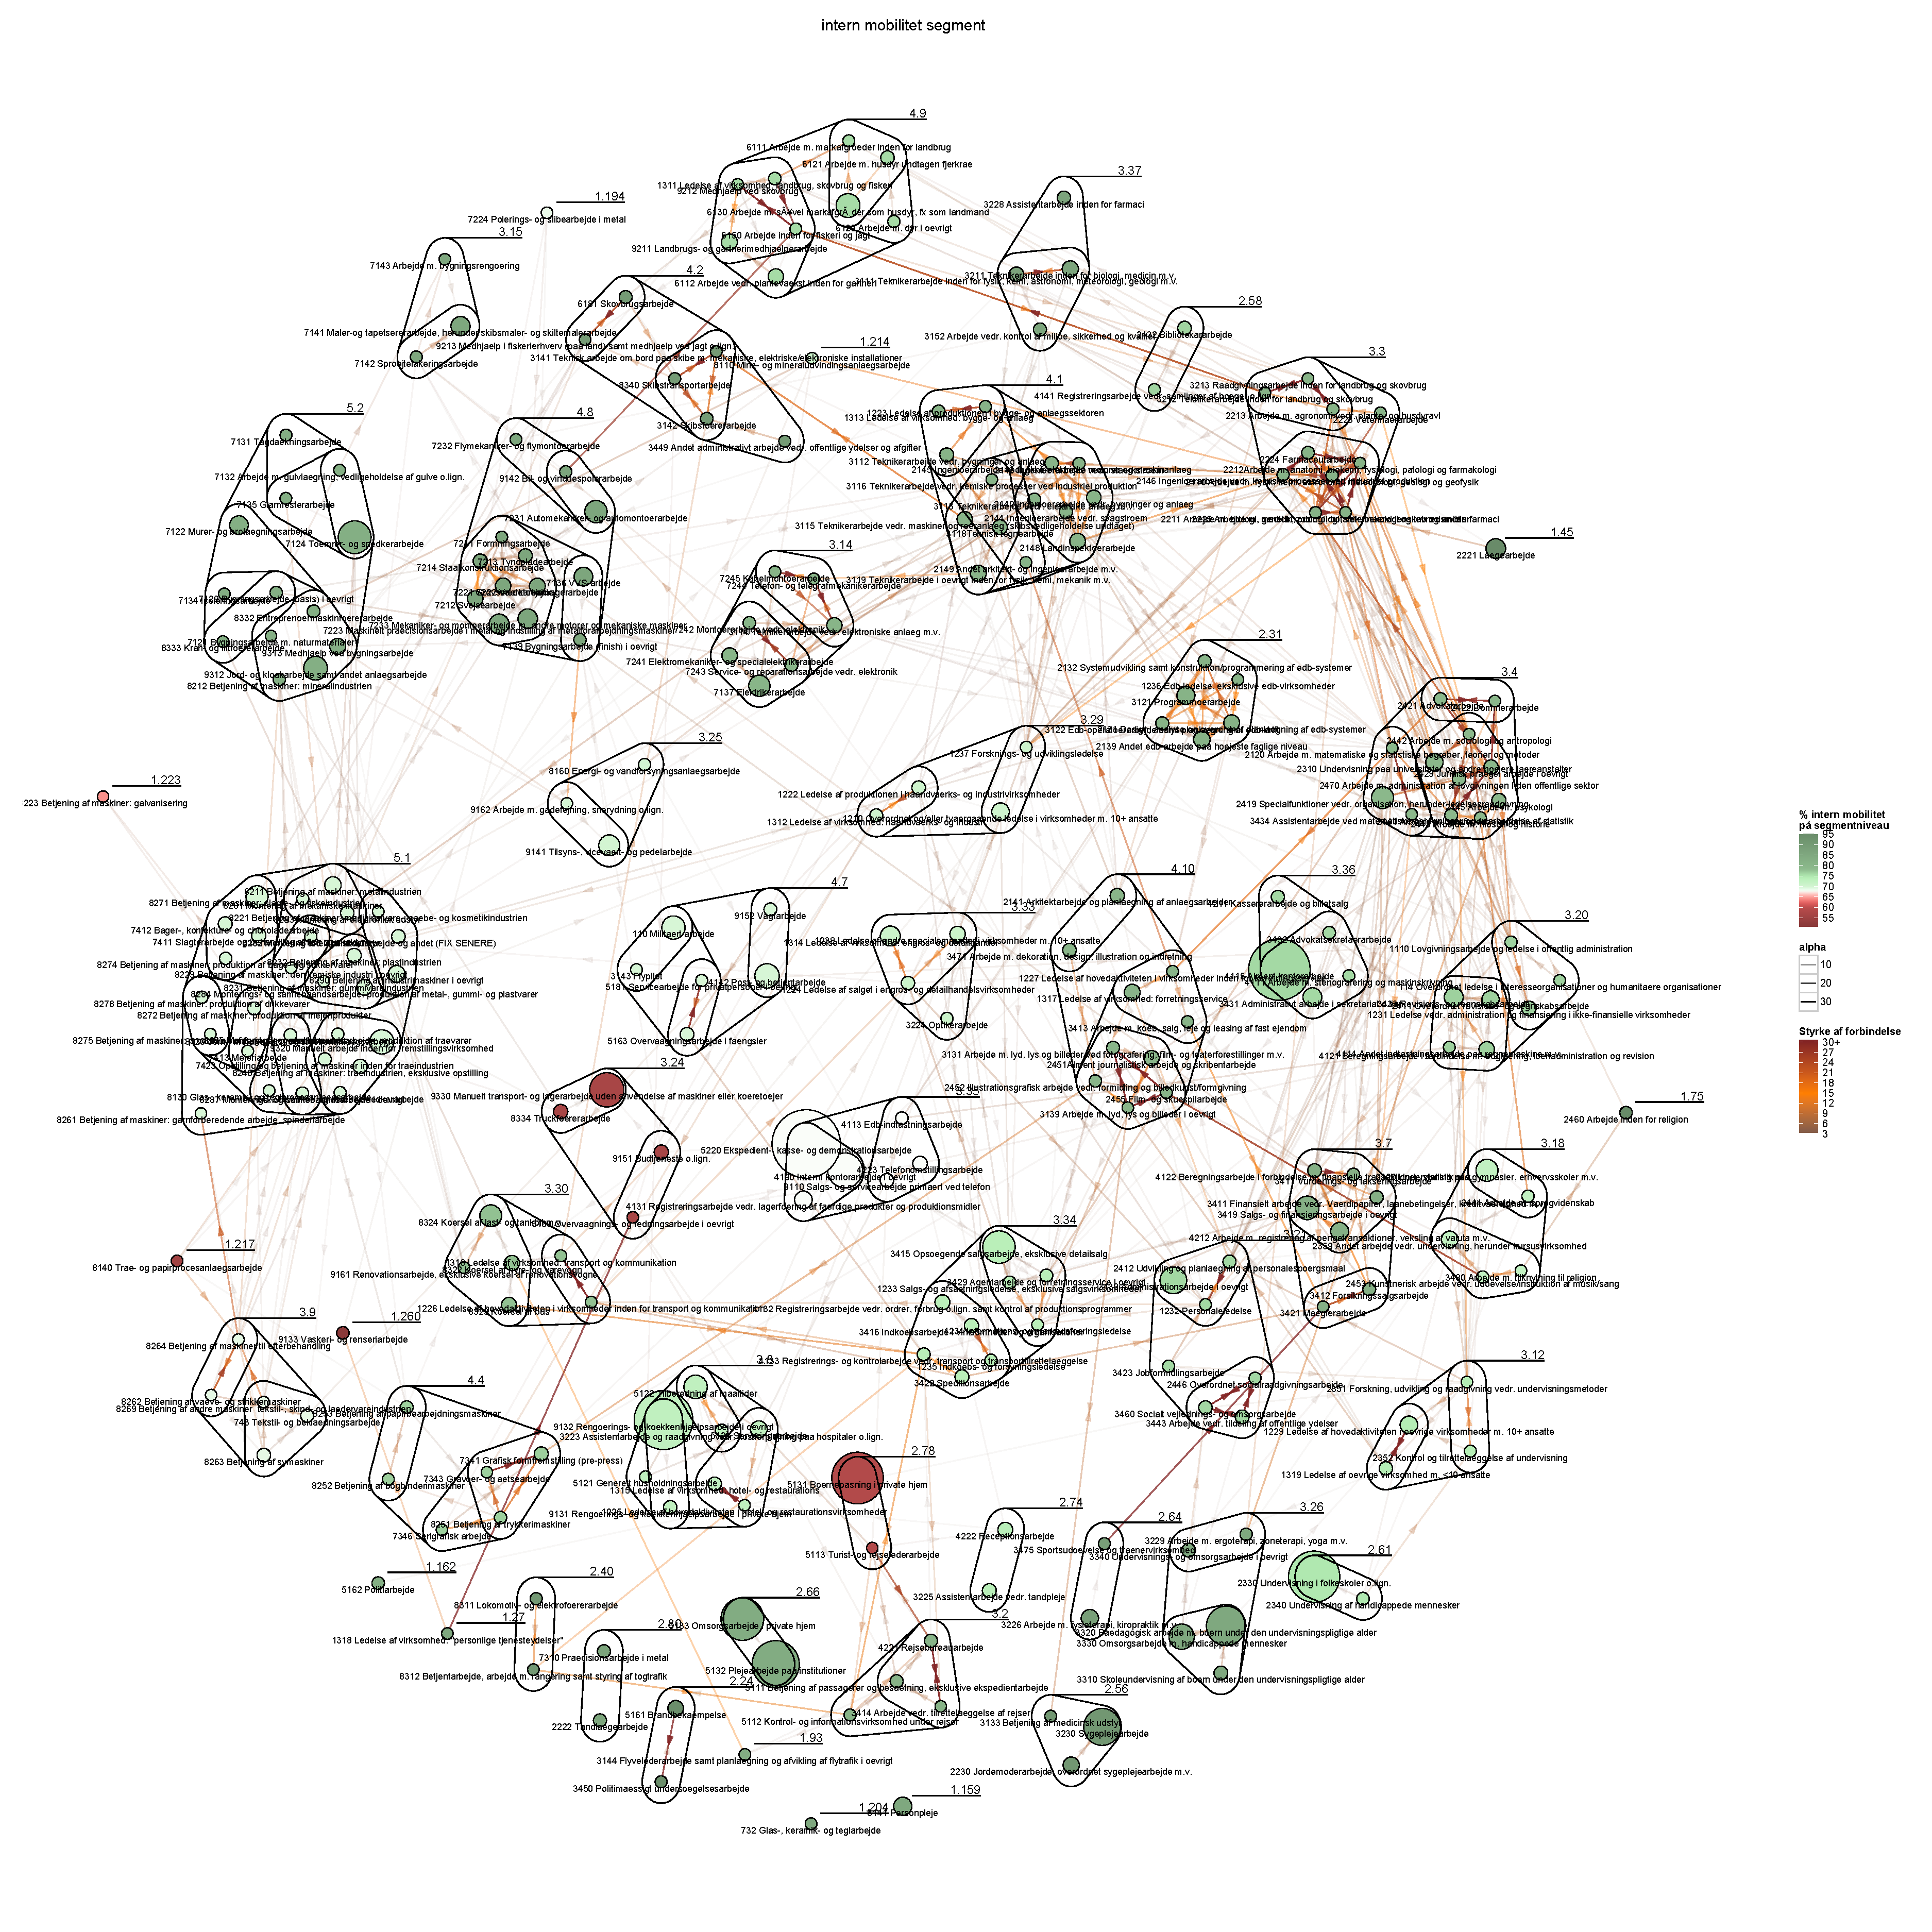
\includegraphics[width=1.0\textwidth]{fig/netvaerkskort/kort_intern_mob_seg.pdf}
	\centerline{ \tiny{Kilde: Nielsen-Gravholt og Begtrup-Bright}}
\end{center}
\end{figure}
\restoregeometry

Det ses på kortet, at nodernes farve går fra mørkerød, til hvid, til mørkegrøn. Mørkerød betyder at klyngen har en intern mobilitet på mellem 50 og 60 \%, mens den derfra og op til 69 \% antager en stadigt svagere lys rød, indtil den er ren hvid ved 70 \%. Derfra og op til 79 \% bliver den stadig mere grøn, for ved 80 \% at være helt mørkegrøn. Da der er tale om en gradient, er skiftet i farve en kontinuer overgang. 

Skiftet i farve er motiveret af min egen vurdering. Der findes ingen tidligere brug af Moneca algoritmen, hvori dette indgående bliver analyseret. Jeg har besluttet mig for, at en mobilitet mellem erhvervene i en klynge på 70 \% og derover, er en fornuftig tærskel%
%
\footnote{Der er ikke er tale om en statistisk test med et vist signifikansniveau, men min egen tentative vurdering. Og selv med de vedtagne signifikansniveauer i statistiske test, eksempelvis p-værdier i en T-test eller en F-test,  der advarer litteraturen om ikke at tolke disse tærskelværdier som skrevet i sten, men som nyttige konventioner (find henvisning, Gujarati og Malchow-Møller \#todo). }%
%
. et skyldes såvel en common sense vurdering, såvel som at nodernes interne mobilitet, det (uaggregerede) niveau 1, er på 68 \%  Det ses at langt de fleste klynger overholder denne beslutningsregel. 5 klynger og 4 noder ligger under 70 \%, dog nogle af dem kun lige under. Det betyder ikke at disse klynger nødvendigvis skal forkastes. Men det holdes i mente, at kvaliteten af klyngedannelsen er lavere end godt er. Jeg vil nu gennemgå disse klynger for at vurdere deres holdbarhed.  

Der kan være to årsager til lav intern mobilitet. Den ene er at beskæftigelserne i disse klynger simpelthen er jobs, der af den ene eller anden årsag er af en type, hvor folk sjældent opholder sig længe i dem. Det kunne man kalde en socialt betinget lav intern mobilitet. Det kunne være ufaglærte jobs, der typisk henvender sig til unge og studerende. Eller ufaglært, sæsonbetinget arbejde, eller jobs der simpelthen er så hårde, eller ansættelserne så usikre, at man ikke bliver i dem længe af gangen. Hvis arbejdet har denne karakter, må man forvente, at de sociale lukningsmekanismer næppe er særlig højtudviklede, hvoraf den mest legitime i moderne samfund må være adgangsgivende uddannelse. Vi vil derfor forvente at finde enten ufaglærte eller fag med lave uddannelsesmæssige krav. Den anden årsag, er en dårlig klyngedannelse ud fra Moneca-algoritmen. 

% Klynge \emak{s5.1} har en intern mobilitet på 69,4 \%. Jeg vil betragte det som acceptabelt, da det ligger så tæt på min tærskelværdi. 
%
\begin{wrapfigure}{r}{6cm}
  \vspace{-20pt}
  \begin{center}
    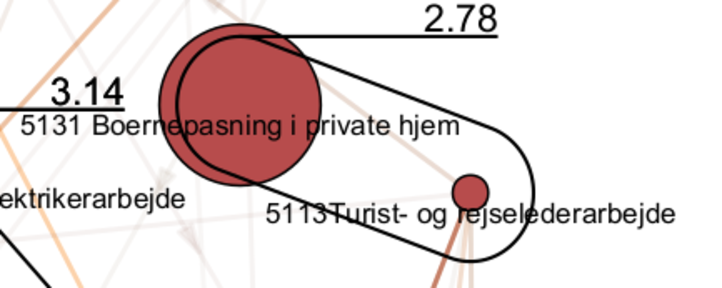
\includegraphics[width=6cm]{fig/segzoom/seg_2_78.pdf}
   \caption{}
   \label{fig_delanalyse1_zoom_2_78}
  \end{center}
  \vspace{-20pt}
\end{wrapfigure}
%
Hvis vi kigger på klynge \emak{s2.78}, kan vi se at den består børnepasning i private hjem, samt turist- og rejseledere. Klyngen har en intern mobilitet på henholdsvis  59 \% og 47 \%, altså ganske lavt sammenlignet med den gennemsnitlige interne mobilitet indenfor erhvervene selv, der er på 68 \%.  Begge jobs er indenfor hovedgruppe 5 i Disco-nomenklaturet, salgs-, service- og omsorgsarbejde. Det er klassificeret som tilhørende færdighedsniveau 2. Det er arbejde, der ifølge Danmarks Statistik er klassificeret som ISCEDs færdighedsniveau 2, hvilket betyder at det kræver uddannelse “på grundniveau” \parencite[tabel 1]{DSTDISCO88}. Det er en klar indikator på at de formelle sociale lukningsmekanismer i erhvervene er begrænsede. 

Der er andre klynger på kortet, hvor uddannelseskravene er lave, men hvor den interne mobilitet er høj. Et nærliggende eksempel er klynge \emak{s2.66}, Der ligeledes befinder sig i hovedgruppe 5, men hvor den interne mobilitet både i klyngen og blandt jobbene selv er meget høj. Børnepasning i private hjem ligger ganske tæt på arbejdsfunktionerne i klynge \emak{s2.66}, faktisk så tæt at de også på et 3-cifret Disco niveau er kategoriseret ens. Men børnepasning i private hjem har tilsyneladende en noget anden social profil. Den interne mobilitet er meget lavere, og den ligger sammen med turist- og rejseleder. 
%
\begin{wrapfigure}{r}{6cm}
  \vspace{-20pt}
  \begin{center}
    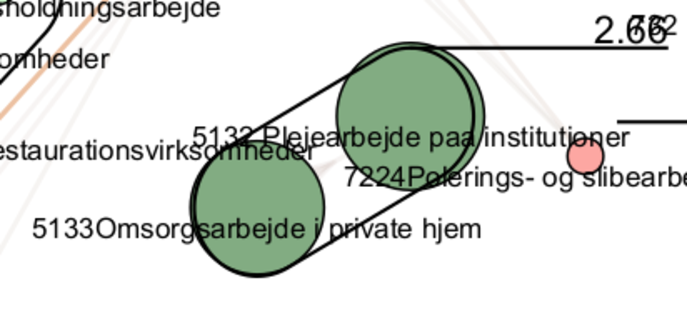
\includegraphics[width=6cm]{fig/segzoom/seg_2_66.pdf}
   \caption{}
   \label{fig_delanalyse1_zoom_2_66}
  \end{center}
  \vspace{-20pt}
\end{wrapfigure}

Der ikke er nævneværdig mobilitet mellem disse to klynger, trods denne enshed. Det får mig til at konkludere, at der trods en vis funktionel enshed mellem børnepasning på en ene side og omsorgsarbejde for ældre mennesker i deres hjem og på institutioner på den anden, er tale om vidt forskellige sociale processser. Den funktionelle enshed er ikke bestemmende for den sociale ditto. Det viser sig også ved at gennemsnitlige alder indenfor klynge \emak{s2.78} er omtrent 37 år.%
%
\footnote{Det også gælder de to jobs i klyngen hver især}%
%
. Klynge \emak{s2.66} har en gennemsnitsalder på 42 $\nicefrac{3}{4}$ år, hvilket er er nærmest identisk med populationsgennemsnitet på 42,3 år. (check hvilken kvartil det befinder sig i på forskermaskinen \#todo). 


















%%%%%%%%%%%%%%%%%%%% noter %%%%%%%%%%%%%%%%%%%%%%%%%%%%%%%%%%%%%%%%%%%


%  Måske skal der laves mere stringent begrebsafklaring om forskel på delmarkeder, segmenter og klynger. 





%%%%%%%%%%%%%%%%%%%%% fragmenter %%%%%%%%%%%%%%%%%%%%%%%%%


% I figur \ref{fig_analyse_deskriptivt_kort_seg_proces} ses denne segmenteringsprocess første 4 stadier/niveauer, repræsenteret visuelt%
% %
% \footnote{Det 5. niveau er ikke medtaget, da det er det endelige niveau. Det vil blive præsenteret og analyseret indgående i resten af afhandlingen.}%
%
% . 
% %
% %
% \newgeometry{left=-0.01cm,bottom=0.1cm}
% \begin{figure}[H]
% \begin{center}
%   \caption{Segmenteringsprocessens første 4 niveauer.}
%   \label{fig_analyse_deskriptivt_kort_seg_proces}
%   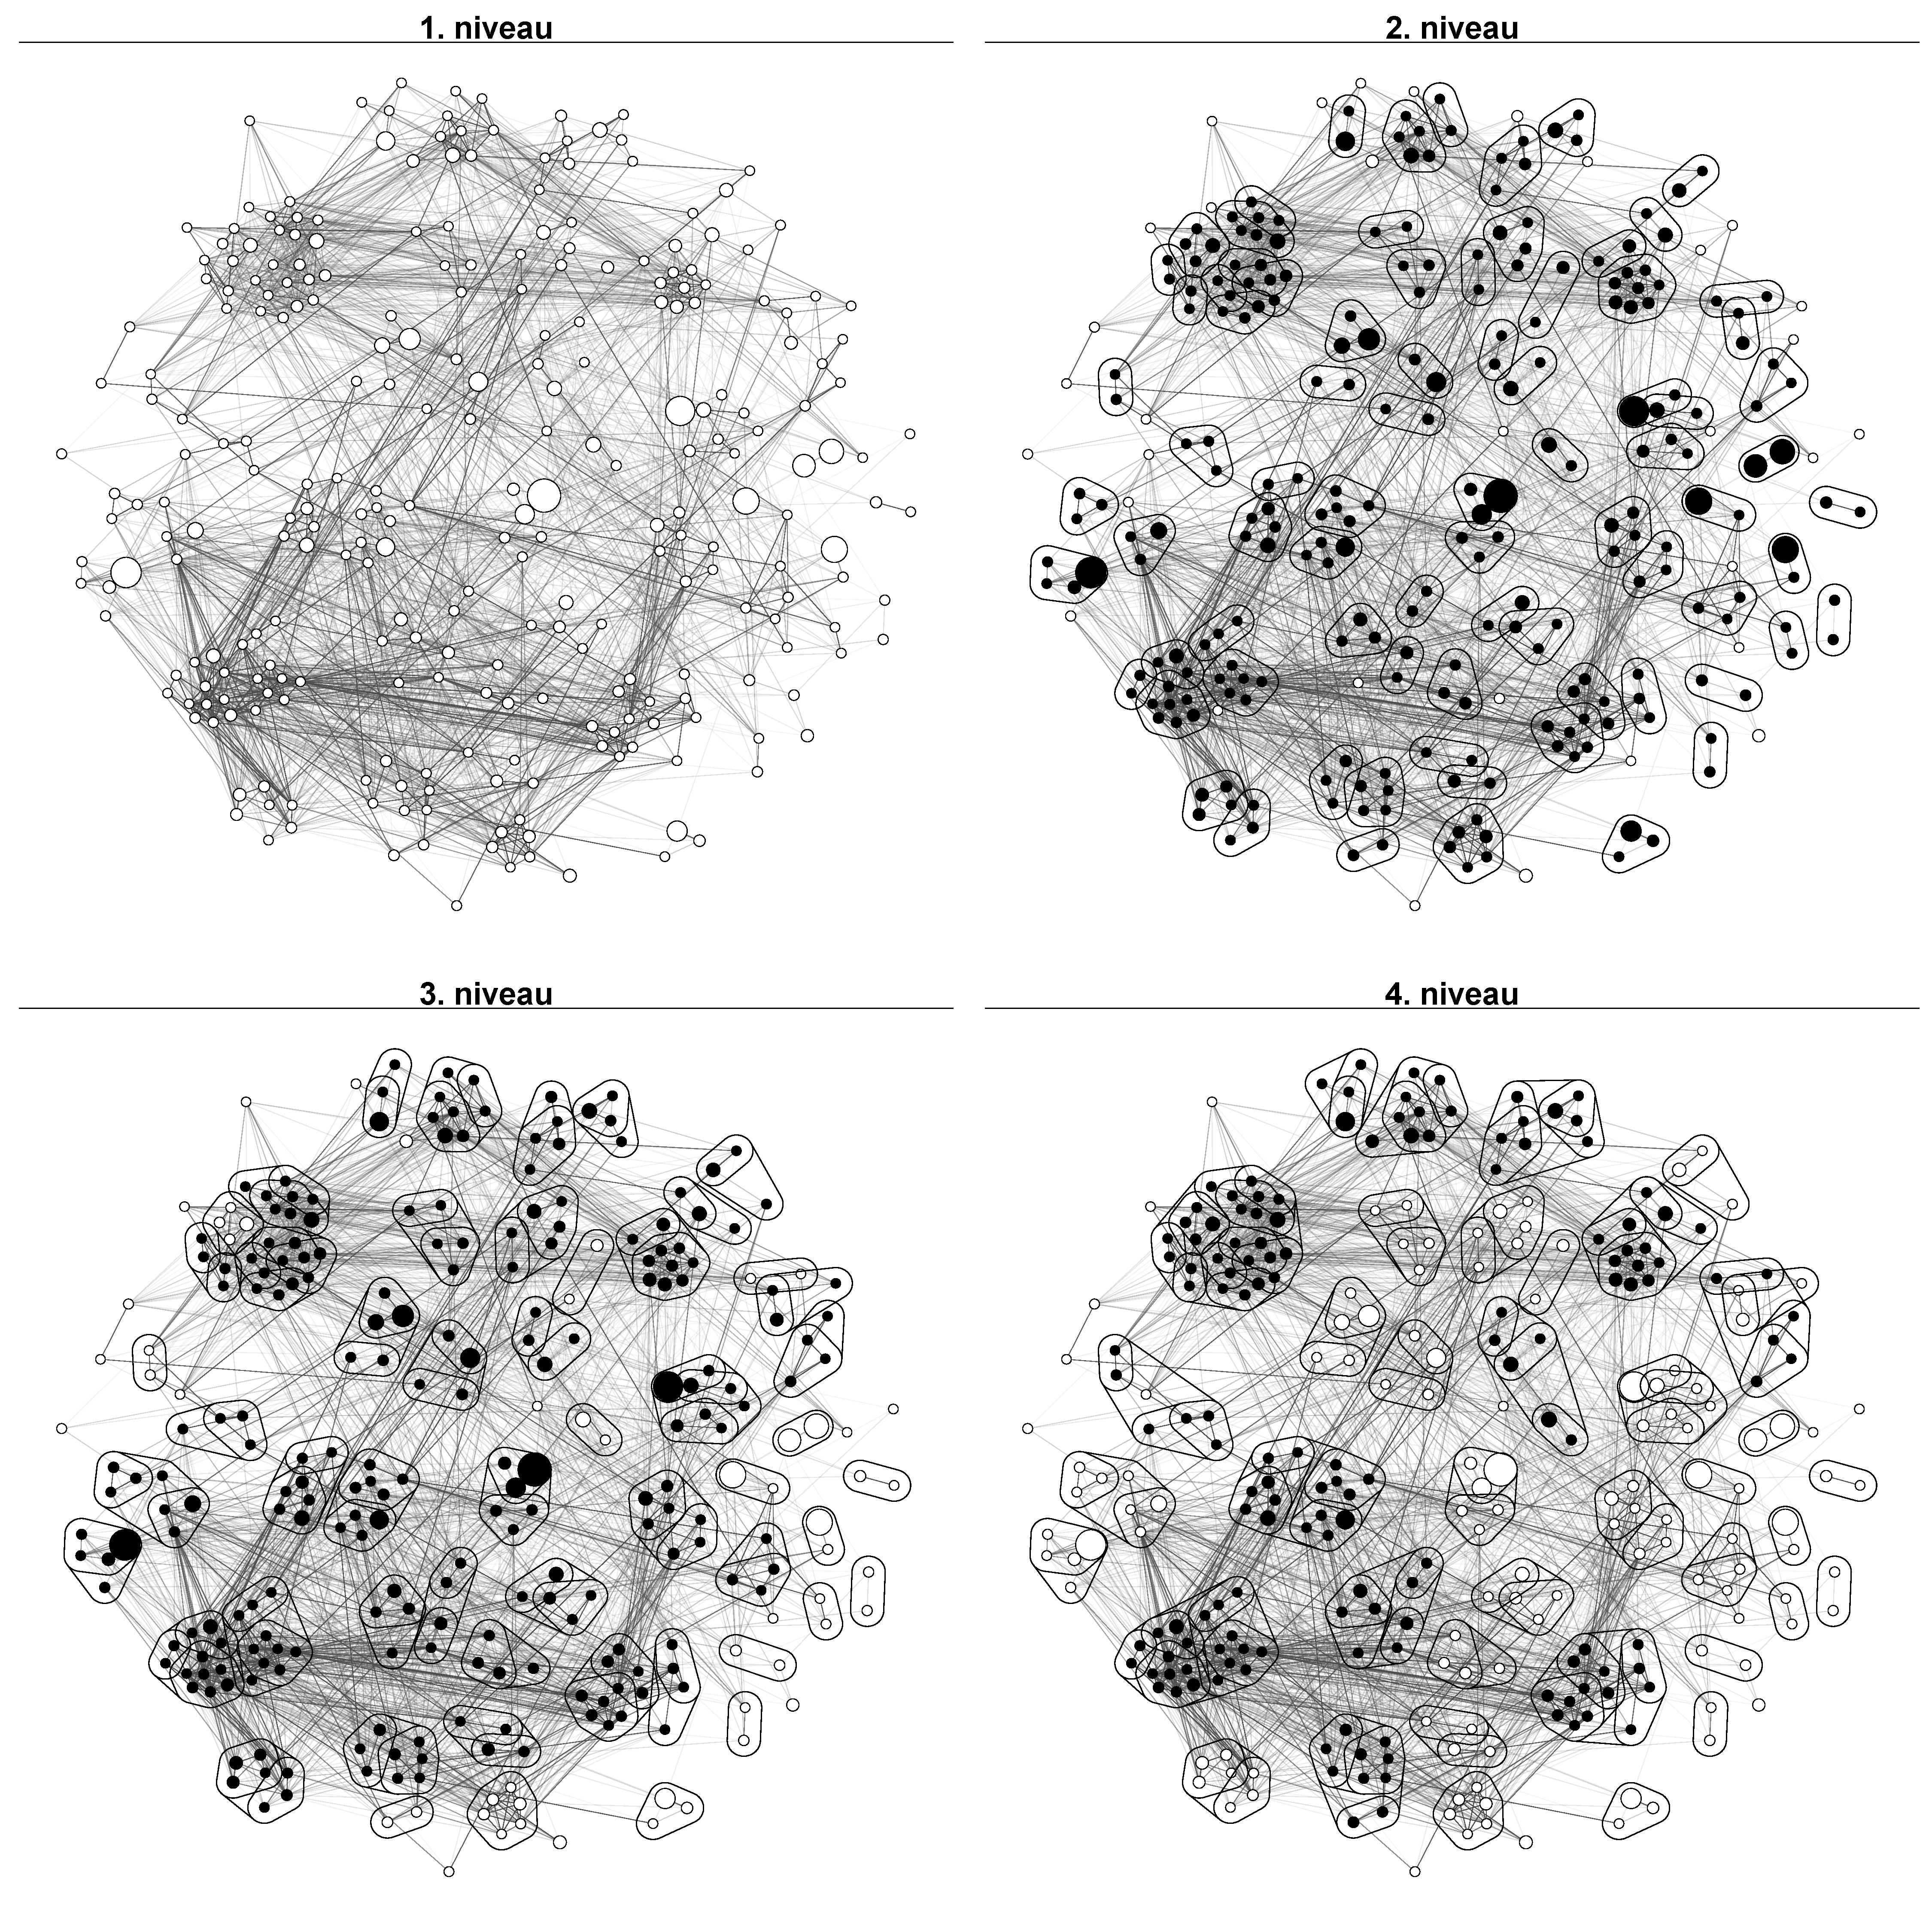
\includegraphics[width=1.0\textwidth]{fig/netvaerkskort/kort_seg_proces.pdf}
%   \centerline{ \tiny{Kilde: Nielsen-Gravholt og Begtrup-Bright}}
% \end{center}
% \end{figure}
% \restoregeometry
% %
% %







